% Auriga theme
% https://github.com/anishathalye/auriga

\documentclass[14pt,aspectratio=169]{beamer}
\usepackage{pgfpages}
\usepackage{fancyvrb}
\usepackage{booktabs,dcolumn}
\usepackage{tikz}
\usetikzlibrary{arrows.meta, positioning, quotes}
\usepackage{pgfplots}

% \ifnotes
% \setbeamertemplate{note page}[plain]
% \setbeameroption{show notes on second screen=right}
% \fi

\usetheme{auriga}
\usecolortheme{auriga}

% define some colors for a consistent theme across slides
\definecolor{red}{RGB}{181, 23, 0}
\definecolor{blue}{RGB}{0, 118, 186}
\definecolor{gray}{RGB}{146, 146, 146}

\title{Historia Económica Argentina}

\author{\underline{Sebastián Freille} \inst{1}}

\institute[shortinst]{\inst{1} IEF-UNC \\ UCC}
\date{}

\AtBeginSection[]{
    \begin{frame}
    \vfill
    \centering
    \begin{beamercolorbox}[sep=8pt,center,shadow=true,rounded=true]{title}
        \usebeamerfont{title}\insertsectionhead\par%
    \end{beamercolorbox}
    \vfill
    \end{frame}
}



\AtBeginSubsection[]{
    \begin{frame}
    \vfill
    \centering
    \begin{beamercolorbox}[sep=6pt,center,shadow=true,rounded=true]{title}
        \usebeamerfont{title}\insertsubsectionhead\par%
    \end{beamercolorbox}
    \vfill
    \end{frame}
}


\AtBeginSubsubsection[]{
    \begin{frame}
    \vfill
    \centering
    \begin{beamercolorbox}[sep=4pt,center,shadow=true,rounded=true]{title}
        \usebeamerfont{title}\insertsubsubsectionhead\par%
    \end{beamercolorbox}
    \vfill
    \end{frame}
}


\begin{document}

{
  % rather than use the frame options [noframenumbering,plain], we make the
  % color match, so that the indicated page numbers match PDF page numbers
  \setbeamercolor{page number in head/foot}{fg=background canvas.bg}
  \begin{frame}
    \titlepage
  \end{frame}
}

  
  \section{Capítulo 2. Los años entre las dos guerras (1914-1945)}


  \subsection{La economía argentina a fines del periodo de oro}


 \begin{frame}\frametitle{El fin de una epoca}
    \begin{itemize}\itemsep 10pt
      \item A principios de la década de 1910, los indicadores
        macroeconómicos de Argentina estaban entre los mejores de su
        historia
        \item La circulacion monetaria tenía un respaldo de 63\%. El
          riesgo país (spread entre bonos locales e internacionales)
          tan bajo como 1.5\%. El déficit público era menor al 20\% de
          los ingresos fiscales. El ratio deuda/PBI era de sólo 35\%.
          \item Muchos historiadores y analistas reconocían el
            potencial para una explosión de crecimiento --pero
            también se resaltaban los peligros
       \end{itemize}
      \end{frame}
  


 \begin{frame}\frametitle{El fin de una epoca (cont.)}
   \begin{block}{El patrón oro para un país periférico}
El patrón oro maximizaba la capacidad de una economia para atraer
inversores externos en periodos florecientes. Pero también lo dejaba
expuesto a potenciales shocks en los términos de intercambio y/o tasas
de interés internacionales. La visión de Alec Ford era que el patrón
oro amplificaba los ciclos económicos --si había una recesión podía
ser amplificada por una contracción monetaria. Se reconocía esta
vulnerabilidad a crisis externas y el estar sujeto a los movimientos
de oro entre los países
     \end{block}
      \end{frame}
  


\begin{frame}\frametitle{El fin de una epoca (cont.)}
    \begin{itemize}\itemsep 10pt
      \item Pocos estaban preparados para sufrir las consecuencias de
        una doble crisis --divisas internacionales y crisis
        financiera.
        \item A principios de 1913, política monetaria contractiva en
          Gran Bretaña causaría problemas en Argentina --a través de
          vinculos de PPP y paridad del interes
          \item Por primera vez en esa década disminuyó la oferta de
            dinero (1913) y luego la base monetaria (1914).
            \item Esto repercutió en una caída de los depósitos en el
              sistema bancario
       \end{itemize}
      \end{frame}
  
      


  \begin{frame}\frametitle{El fin de una epoca (cont.)}
\begin{figure}[htbp]\vspace{0cm}
  \centering
  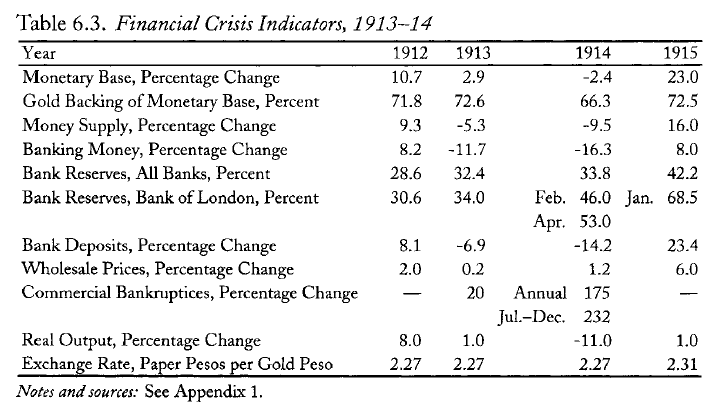
\includegraphics[scale=0.5]{uni1_mon17}
  \caption[bpe]{Del crecimiento a la transición, 1912-15. Fuente:
    Della Paolera and Taylor (2001)}
  \label{fig:uni1_01}
\end{figure} 
  \end{frame}



  
\begin{frame}\frametitle{El fin de una epoca (cont.)}
    \begin{itemize}\itemsep 10pt
      \item Empezaba a instalarse una presión deflacionaria (importada
        desde Europa) que luego afectaría a muchos indicadores del
        sistema bancario y financiero
        \item En una deflación suelen pasar varias cosas que afectan a
          los bancos:
          \begin{itemize}\itemsep 10pt \medskip
            \item cambio marcado en el valor relativo de
          activos y pasivos --agentes buscan liquidez en forma de
          efectivo versus depósitos (pasivo) en
          lugar de mantener activos ilíquidos (activos) 
          \item cambia el ratio de obligaciones monetarias (dinero amplio) a reservas
            $\longrightarrow$ el problema aqui era si el público
            prefería dinero en mano a un depósito, el multiplicador
            monetario baja [$mm=\frac{1+e}{r+e}$]
          \end{itemize}
       \end{itemize}
      \end{frame}

      
\begin{frame}\frametitle{El fin de una epoca (cont.)}
    \begin{itemize}\itemsep 10pt
      \item Es así como la economía se mueve de una deflación a una
        crisis financiera (sustitucion de depositos por pesos). Las
        reservas como fraccion de los depósitos bajan cada vez mas y
        es necesario inyectar liquidez en el sistema
        \item Como podemos recordar, la CdC tenía vedadas por ley la
          función de \textbf{prestamista de última instancia} y para
          el caso tampoco de ninguna otra institucion.
          \item Leccion $\longrightarrow$ \textbf{trade-off} entre
            convertibilidad interna --estabilizar el sistema
            financiero local- y convertivilidad externa --mantener el
            estandar monetario garante del valor de la moneda
          \end{itemize}
      \end{frame}
      
      
      
  
  \subsection{La Primera Guerra Mundial (1914-1918): Efectos sobre la economía
    argentina y la política econónomica local}


   \begin{frame}\frametitle{El fin de una epoca}
    \begin{itemize}\itemsep 10pt
      \item El inicio de la Primera Guerra Mundial (1GM) el 28 de julio de
        1914 marcó decididamente el fin de una época de paz y
        prosperidad $\longrightarrow$ conforman Triple Alianza
        --Alemania, Imperio Austro-húngaro e Italia- y Triple Entente
        --Francia, Gran Bretaña y Rusia.
        \item El impacto en la economía fue casi inmediato
          $\longrightarrow$ principales bolsas cerraron sus puertas;
          se abandonó el compromiso del patrón oro; y se restringió
          fuertemente la movilidad del oro
       \end{itemize}
      \end{frame}


 \begin{frame}\frametitle{El fin de una epoca (cont.)}
    \begin{itemize}\itemsep 10pt
      \item Argentina, en tanto economía pequeña y abierta, sufriría
        las consecuencias de estos cambios --la cuenta capital se
        redujo casi un 50\% entre 1913 y 1914. La balanza comercial
        fue positiva pero por una fenomenal contracción de las M (35\%).
        \item La balanza de  pagos que había sido positiva todos los
          años desde 1900 fue deficitaria por primera vez --cuenta
          capital negativa de 1914 a 1918
          \item Los principales movimientos de la balanza comercial
            fueron debido a \textbf{cantidades} y no precios --tanto
            $P_{X}$ como $P_{M}$ fueron crecientes en este periodo
            [como era de esperarse]
       \end{itemize}
      \end{frame}
      


       \begin{frame}\frametitle{El fin de una epoca (cont.)}
\begin{figure}[htbp]\vspace{0cm}
  \centering
  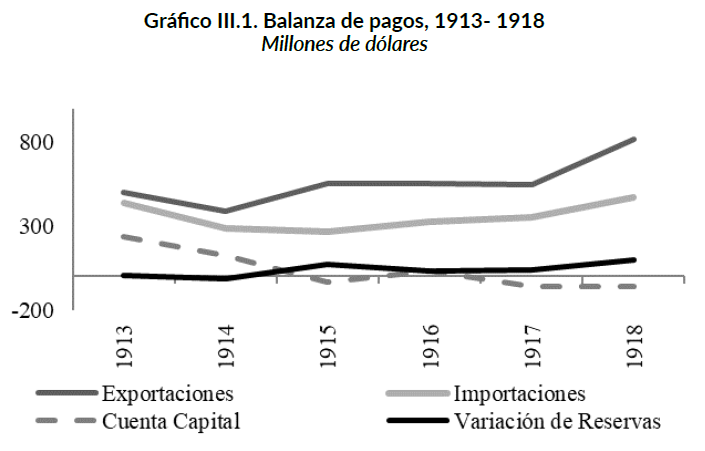
\includegraphics[scale=0.5]{uni2_1gm01}
  \caption[bpe]{Evolución balanza de pagos, 1913-18. Fuente:
    Gómez (2018)}
  \label{fig:uni1_01}
\end{figure} 
  \end{frame}


  \begin{frame}\frametitle{El fin de una epoca (cont.)}
\begin{figure}[htbp]\vspace{0cm}
  \centering
  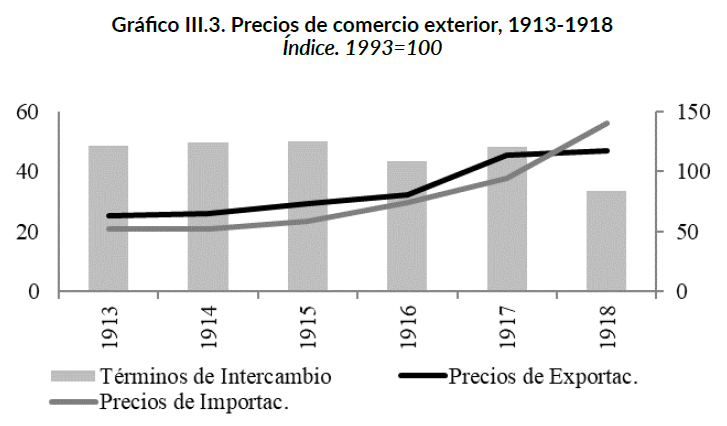
\includegraphics[scale=0.5]{uni2_1gm02}
  \caption[bpe]{Evolución precios de M y X, 1913-18. Fuente:
    Gómez (2018)}
  \label{fig:uni1_01}
\end{figure} 
  \end{frame}




 \begin{frame}\frametitle{El fin de una epoca (cont.)}
    \begin{itemize}\itemsep 10pt
      \item Salvo entre 1913-14, el valor de exportaciones subió entre
        1914 y 1918 --efecto precio ya que cantidades cayeron en
        varios años (malas cosechas)
        \item Algo similar pasó con las M --subieron por efecto
          precio- aunque las cantidades cayeron en todos los años
          \item El principal dato es la permanencia de las M por abajo
            de las X --esto permitió un saldo positivo de la balanza
            de pagos hacia la salida de la 1GM
       \end{itemize}
      \end{frame}
      

 \begin{frame}\frametitle{El fin de una epoca (cont.)}
\begin{figure}[htbp]\vspace{0cm}
  \centering
  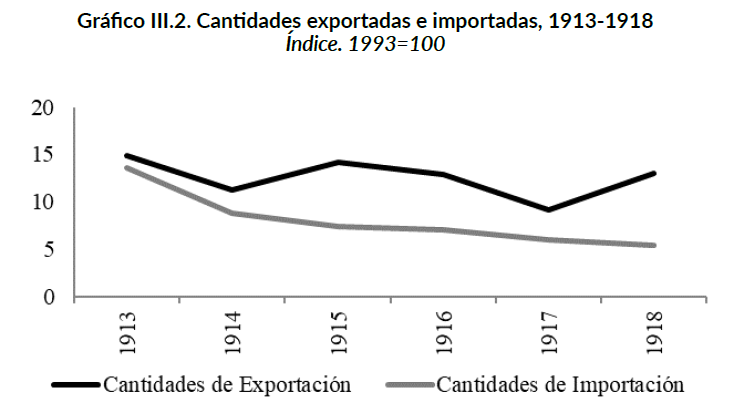
\includegraphics[scale=0.5]{uni2_1gm03}
  \caption[bpe]{Evolución cantidades de M y X, 1913-18. Fuente:
    Gómez (2018)}
  \label{fig:uni1_01}
\end{figure} 
  \end{frame}




 \begin{frame}\frametitle{Los cambios institucionales}
    \begin{itemize}\itemsep 10pt
      \item La primera y más urgente medida de política económica fue
        el decreto de \textbf{feriado bancario} (incluida CdC) de una semana
        seguida de un \textbf{paquete de leyes de emergencia}
        \item Establecian prórrogas (30 días) para cumplimiento de obligaciones
          de particulares --excepto obligaciones tributarias de
          cualquier nivel
          \item Prórroga también aplicable a obligaciones de bancos
            con depositantes $\longrightarrow$ sólo pagarían hasta el
            20\% de depósitos exigibles
       \end{itemize}
      \end{frame}


       \begin{frame}\frametitle{Los cambios institucionales (cont.)}
    \begin{itemize}\itemsep 10pt
      \item El oro proveniente de transacciones comerciales sería
        \textbf{depositado en las legaciones argentinas} en el exterior
        \item De este modo, las legaciones argentinas se convertían en
          sucursales de la CdC.
          \item CdC podía emitir apenas se depositara nuevo oro en las
            legaciones en la misma relación 2.27 a 1 fijada por la ley
            de Conversión (1899)
       \end{itemize}
      \end{frame}
      

  \begin{frame}\frametitle{Los cambios institucionales (cont.)}
    \begin{itemize}\itemsep 10pt
      \item En tercer lugar, se decretó la \textbf{suspensión de la
        convertibilidad} $\longrightarrow$ primero por 30 dias
      prorrogables por otros 30 días y luego por tiempo indefinido
      \item En octubre de 194 se suspende el compromiso de convertir
        los pesos papel a pesos oro (en paridad fija)
        $\longrightarrow$ \textbf{sistema de papel moneda
          inconvertible}
                 \end{itemize}
      \end{frame}
      


  \begin{frame}\frametitle{Los cambios institucionales (cont.)}
    \begin{itemize}\itemsep 10pt
      \item Se autorizaba al PE a prohibir parcial/totalmente la
        exportacion de metálico  \textbf{control de cambios}
        mientras subsistiera el estado de guerra $\longrightarrow$
        significaba de derecho el fin de la libre movilidad de K
        \item No se utilizó esta prerrogativa durante el conflicto
          $\longrightarrow$ oro siguió entrando y saliendo según saldo
          de BP
                 \end{itemize}
      \end{frame}


       \begin{frame}\frametitle{Los cambios institucionales (cont.)}
    \begin{itemize}\itemsep 10pt
      \item Un cambio clave fue la autorización al BNA
el uso del Fondo de Conversión y a la CdC para
\textbf{otorgar redescuentos}, dado un respaldo de 40\% de la BM en metálico
\item Los redescuentos por tanto podían hacerse: 1) BNA podia hacer
  redescuentos de otros bancos fijando plazos e interés (continuidad);
  2) BNA podía dar a la CdC sus propios documentos o los de otros
  bancos (cambio); 3) CdC podía crear dinero primario a cambio de
  docuemntos comerciales presentados por el BNA
  \item Cambio fundamental $\longrightarrow$ CdC podía emitir contra
    redescuentos (aunque no lo hizo en la práctica)
                 \end{itemize}
      \end{frame}

      

  \begin{frame}\frametitle{Funciones banco-centralistas: CdC}
    \begin{itemize}\itemsep 10pt
      \item CdC no tenia obligacion de convertir pesos papel a pesos
        oro a la tasa de 2.27 por 1 --se alejó del principio de la
        \textit{Currency School} y también del patrón oro de una sóla
        via
        \item Tanto en el grafico como en la tabla puede observarse
          que durante este periodo el gobierno no siguió ninguno de
          los dos patrones rectores --\textit{Currency School} o
          \textit{patrón oro de una sola via}.
          \item Patrón de \textbf{autoregulación} $\longrightarrow$ si
            reservas disminuían, la BM constante; si aumentaban, la BM
            constante. 
                 \end{itemize}
      \end{frame}

      

 \begin{frame}\frametitle{Funciones banco-centralistas: CdC (cont.)}
\begin{figure}[htbp]\vspace{0cm}
  \centering
  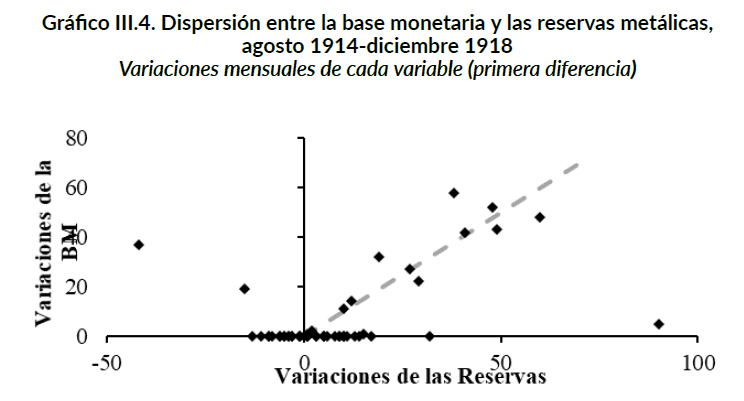
\includegraphics[scale=0.5]{uni2_1gm04}
  \caption[bpe]{Base monetaria y reservas metálicas, 1914-18. Fuente:
    Gómez (2018)}
  \label{fig:uni1_01}
\end{figure} 
  \end{frame}


 \begin{frame}\frametitle{Funciones banco-centralistas: CdC}
    \begin{itemize}\itemsep 10pt
      \item CdC no tenia obligacion de convertir pesos papel a pesos
        oro a la tasa de 2.27 por 1 --se alejó del principio de la
        \textit{Currency School} y también del patrón oro de una sóla
        via
        \item Tanto en el grafico como en la tabla puede observarse
          que durante este periodo el gobierno no siguió ninguno de
          los dos patrones rectores --\textit{Currency School} o
          \textit{patrón oro de una sola via}.
          \item Patrón de \textbf{autoregulación} $\longrightarrow$ si
            reservas disminuían, la BM constante; si aumentaban, la BM
            constante. 
                 \end{itemize}
      \end{frame}

  


 \begin{frame}\frametitle{Funciones banco-centralistas: CdC (cont.)}
\begin{figure}[htbp]\vspace{0cm}
  \centering
  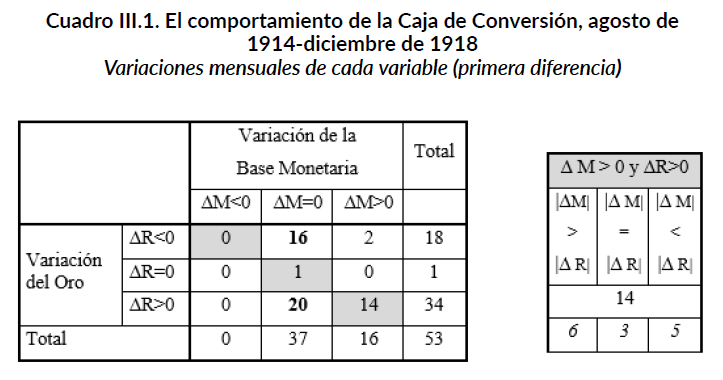
\includegraphics[scale=0.5]{uni2_1gm05}
  \caption[bpe]{Variaciones de BM y Oro según cantidad de meses, 1914-18. Fuente:
    Gómez (2018)}
  \label{fig:uni1_01}
\end{figure} 
  \end{frame}


       \begin{frame}\frametitle{Funciones banco-centralistas: CdC (cont.)}
    \begin{itemize}\itemsep 10pt
      \item El comportamiento del \textbf{tipo de cambio} quedaba de
        esta manera determinado por las acciones del gobierno
        $\longrightarrow$ $\Delta R<0  \Rightarrow \Delta BM=0
        \Rightarrow Depreciación (suba del TDC) $ mientras que $\Delta R>0
        \Rightarrow \Delta BM=0 \Rightarrow Apreciación (baja del
        TDC)$
        \item Se utilizaron 20 millones de pesos oro del FDC para
          salvar al sistema bancario (sin incluir al BNA)
          $\longrightarrow$ pero la acción bancocentralista no fue del
          BNA sino de la CdC (aun sin emitir usó el FDC) --mermó el
          respaldo de la totalidad de la BM (de 73\% a 66\%)
                 \end{itemize}
      \end{frame}
  
  
 \begin{frame}\frametitle{Funciones banco-centralistas: CdC (cont.)}
\begin{figure}[htbp]\vspace{0cm}
  \centering
  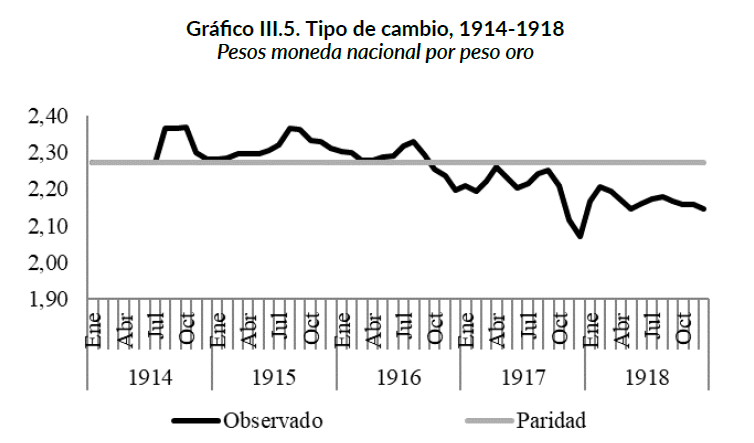
\includegraphics[scale=0.5]{uni2_1gm06}
  \caption[bpe]{Tipo de cambio 1914-1918. Fuente:
    Gómez (2018)}
  \label{fig:uni1_01}
\end{figure} 
  \end{frame}



 \begin{frame}\frametitle{El sistema bancario}
    \begin{itemize}\itemsep 10pt
      \item Al estallar la 1GM hubo una mayor demanda por liquidez en
        Argentina --retiro de depósitos (corrida) en casi todos los bancos pero
        en diferente magnitud
        \item La razón $C/D$ aumento casi un 30\% en segundo semestre
          de 1914 --bancos nacionales sufrieron más que extranjeros y
          BNA
          \item Pero el sistema bancario estaba fuerte y revitalizado
            por la ayuda de los redescuentos --no hubo problemas
            significativos de liquidez (caída del 20\% a nivel del sistema)
                 \end{itemize}
      \end{frame}
  


      
 \begin{frame}\frametitle{Funciones banco-centralistas: CdC (cont.)}
\begin{figure}[htbp]\vspace{0cm}
  \centering
  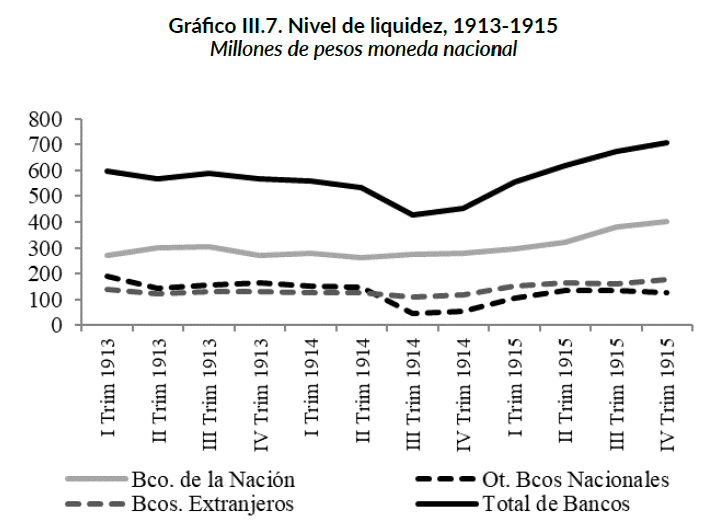
\includegraphics[scale=0.5]{uni2_1gm07}
  \caption[bpe]{Nivel de liquidez sistema bancario 1913-1915. Fuente:
    Gómez (2018)}
  \label{fig:uni1_01}
\end{figure} 
  \end{frame}



 \begin{frame}\frametitle{El sistema bancario}
    \begin{itemize}\itemsep 10pt
      \item Al estallar la 1GM hubo una mayor demanda por liquidez en
        Argentina --retiro de depósitos (corrida) en casi todos los bancos pero
        en diferente magnitud
        \item La razón $C/D$ aumento casi un 30\% en segundo semestre
          de 1914 --bancos nacionales sufrieron más que extranjeros y
          BNA
          \item Pero el sistema bancario estaba fuerte y revitalizado
            por la ayuda de los redescuentos --no hubo problemas
            significativos de liquidez (caída del 20\% a nivel del sistema)
                 \end{itemize}
               \end{frame}
               

 \begin{frame}\frametitle{El sistema bancario (cont.)}
    \begin{itemize}\itemsep 10pt
      \item Luego de este primer período de zozobra --1913 a 1915- la
        tasa de crecimiento de los depósitos fueron de las más altas
        de la historia --21.4\% para el BNA y 36.2\% para el resto de
        bancos
      \item Recuperación de los
        depósitos no estuvo desligada del aumento de la BP despues de 1914.
       \item  Liquidez casi a niveles del período 1900-1914 --ratio
          $R/D$ levemente por debajo. Sistema bancario se mantuvo
          sólido y líquido.
      \end{itemize}
               \end{frame}
               

               
      
 \begin{frame}\frametitle{El sistema bancario (cont.)}
\begin{figure}[htbp]\vspace{0cm}
  \centering
  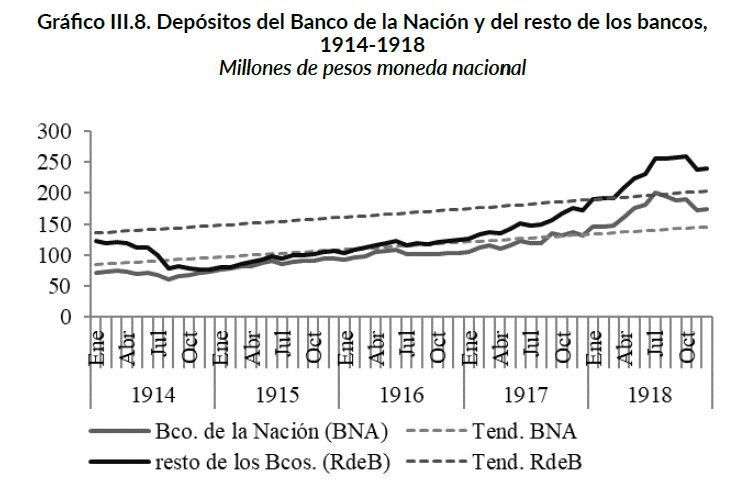
\includegraphics[scale=0.5]{uni2_1gm08}
  \caption[bpe]{Depósitos del sistema bancario, 1914-1918. Fuente:
    Gómez (2018)}
  \label{fig:uni1_01}
\end{figure} 
  \end{frame}
               

\begin{frame}\frametitle{El Estado}
    \begin{itemize}\itemsep 10pt
      \item Inevitablemente, la situación fiscal empeoro en 1914
        --resultado primario y financiero negativos (este ultimo de
        3\% del PBI).
        \item Si bien la situación mejoró en los años siguientes
          recién en 1918 se volvió a superavit primario --el
          financiero era aun negativo
          \item Contrario a lo que se puede pensar, hubo gran
            disciplina fiscal --$GP/PBI$ cayó en todos los años; pero
            también cayeron fuerte los ingresos.
      \end{itemize}
               \end{frame}
               

 \begin{frame}\frametitle{El Estado (cont.)}
\begin{figure}[htbp]\vspace{0cm}
  \centering
  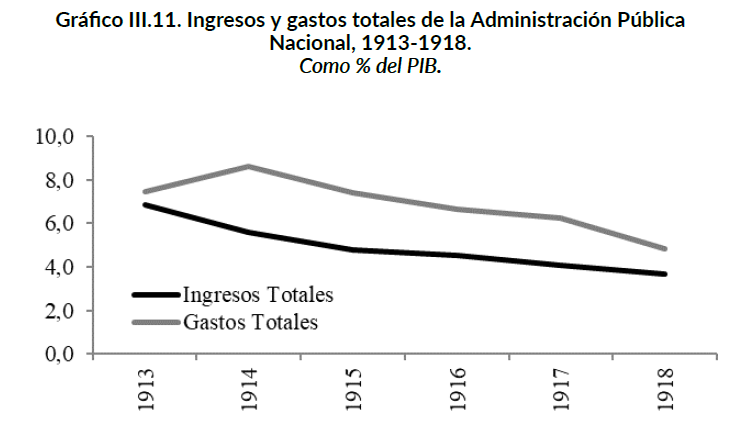
\includegraphics[scale=0.5]{uni2_1gm09}
  \caption[bpe]{Ingresos y gastos de la APN (\% del PBI), 1914-1918. Fuente:
    Gómez (2018)}
  \label{fig:uni1_01}
\end{figure} 
  \end{frame}
               
  

 \begin{frame}\frametitle{Funciones banco-centralistas: BNA}
    \begin{itemize}\itemsep 10pt
      \item El BNA sólo cumplió la función banco-centralista en el año
        1914 --los redescuentos del BNA representaron cerca del 20\%
        de las reservas de los bancos
        \item El sistema bancario entonces no dependió para su
          subsistencia de la ayuda del BNA
                 \end{itemize}
      \end{frame}



      \begin{frame}\frametitle{Funciones banco-centralistas: BNA (cont.)}
\begin{figure}[htbp]\vspace{0cm}
  \centering
  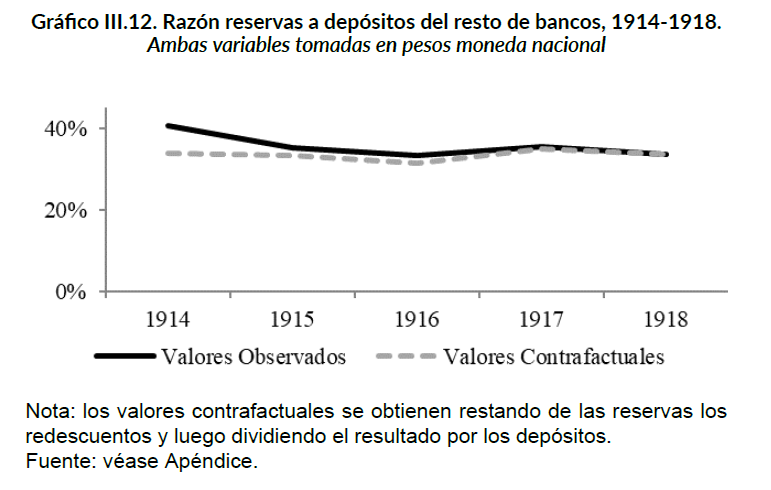
\includegraphics[scale=0.5]{uni2_1gm10}
  \caption[bpe]{Razón reservas/depósitos, Observada y contrafactual, 1914-1918. Fuente:
    Gómez (2018)}
  \label{fig:uni1_01}
\end{figure} 
  \end{frame}



   

 \begin{frame}\frametitle{Funciones banco-centralistas: BNA (cont.)}
    \begin{itemize}\itemsep 10pt
      \item En este periodo el BNA hizo \textbf{financiamiento de
          corto plazo} al Estado $\longrightarrow$ dos ``líneas''
        principales 1) ordinario --Cuenta de Tesorería General-;
        2) extraordinario --Letras de Tesorería.
        \item Letras emitidas a plazo de 180 dias $\longrightarrow$
          bancos ``descontaban'' (compraban) Letras al Estado dandole
          fondos a cambio; y bancos luego solicitaban adelantos al BNA
          dando en caución las Letras
          \item Estrategia $\longrightarrow$ el BNA no tenía deuda
            directa del Estado sino deuda interbancaria
                 \end{itemize}
      \end{frame}


 \begin{frame}\frametitle{Funciones banco-centralistas: BNA (cont.)}
    \begin{itemize}\itemsep 10pt
      \item Estas operaciones crecieron de manera importante mietras
        el Estado se financiaba --
                 \end{itemize}
      \end{frame}
      

  

 \begin{frame}\frametitle{Funciones banco-centralistas: BNA (cont.)}
\begin{figure}[htbp]\vspace{0cm}
  \centering
  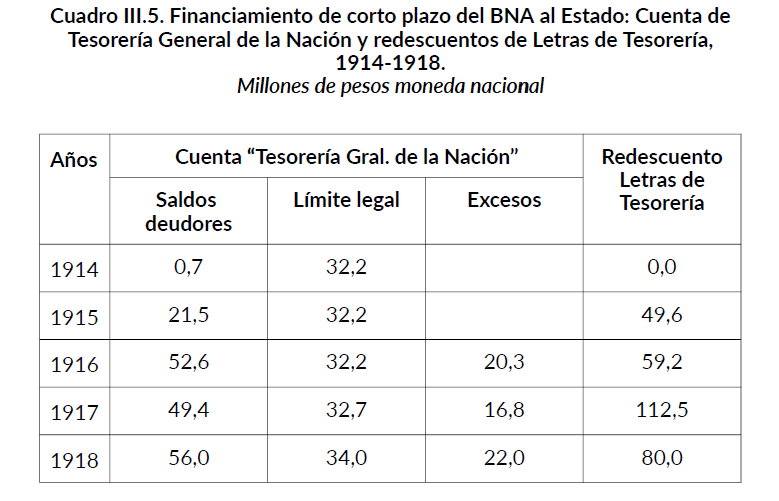
\includegraphics[scale=0.5]{uni2_1gm11}
  \caption[bpe]{Cuentas de financiamiento bancario al Estado, 1914-1918. Fuente:
    Gómez (2018)}
  \label{fig:uni1_01}
\end{figure} 
  \end{frame}


 \begin{frame}\frametitle{Funciones banco-centralistas: BNA (cont.)}
    \begin{itemize}\itemsep 10pt
      \item Pero también hubo \textbf{financiamiento a largo plazo}
        del BNA al Estado $\longrightarrow$ 1) fondos públicos y 2)
        préstamos oficiales
      \item Los primeros fueron crecientes pero sin exceder el
          límite legal (20\% de los fondos del BNA)
          \item Los segundos eran préstamos destinados a ciertos
            destinos --cancelar deuda con bancos de Nueva York en
            1917-; --préstamo del gobierno argentino a potencias
            aliadas para adquirir sobrante de cosechas en 1918                 \end{itemize}
      \end{frame}
      
  

 \begin{frame}\frametitle{Funciones banco-centralistas: BNA (cont.)}
\begin{figure}[htbp]\vspace{0cm}
  \centering
  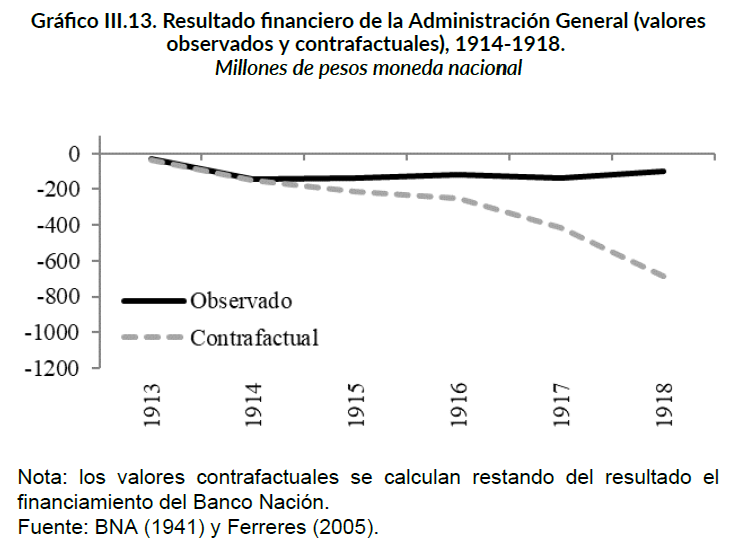
\includegraphics[scale=0.5]{uni2_1gm12}
  \caption[bpe]{Resultado financiero de la APN, Observado y contrafactual, 1914-1918. Fuente:
    Gómez (2018)}
  \label{fig:uni1_01}
\end{figure} 
  \end{frame}
      


 \begin{frame}\frametitle{Funciones banco-centralistas: BNA (cont.)}
    \begin{itemize}\itemsep 10pt
      \item ¿A qué debió renunciar el BNA para acomodar el déficit
        fiscal del gobierno?
      \item Se construyen dos contrafactuales --sumar a las reservas
        del BNA los redescuentos de carteras de otros bancos
        [contrafactual 1]; sumar a las reservas del BNA el
        financiamiento al sector publico (CP y LP) [contrafactual 2]
        \item El \textbf{sacrificio por redescuentos de documentos de
            otros bancos} fue insignificante. El \textbf{sacrificio
            por financiamiento al Estado} fue importante
          \item De no haberse financiado al Estado, cociente $R/D$
            igual a 69\% (23 puntos mas)
      \end{itemize}
      \end{frame}


      
 \begin{frame}\frametitle{Funciones banco-centralistas: BNA (cont.)}
\begin{figure}[htbp]\vspace{0cm}
  \centering
  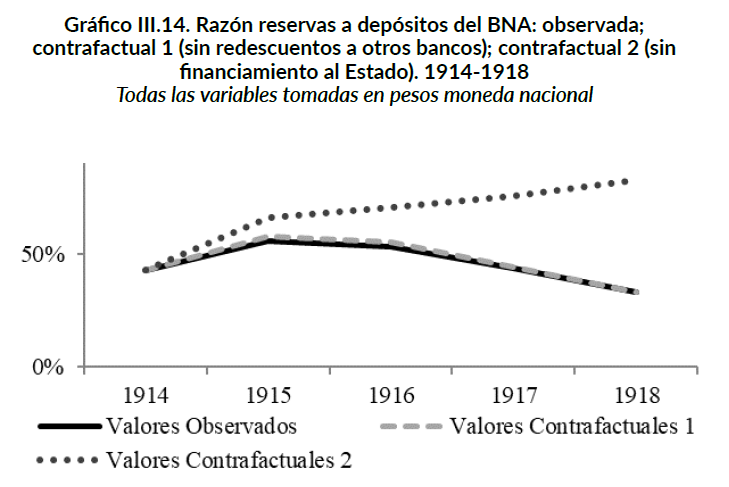
\includegraphics[scale=0.5]{uni2_1gm13}
  \caption[bpe]{Ratio $R/D$ de BNA con y sin contrafactuales, 1914-1918. Fuente:
    Gómez (2018)}
  \label{fig:uni1_01}
\end{figure} 
  \end{frame}



  
 \begin{frame}\frametitle{Resumiendo}
    \begin{itemize}\itemsep 10pt
    \item Durante toda la 1GM, la BP fue positiva salvo por 1914.
      \item La politica económica local se anticipó y actuó
        rapidamente --1) suspensión de convertibilidad; 2) uso del
        FDC; 3) autorizaba redescuentos a la CdC.
        \item Se utilizó un modelo diferente --autoregulación- en que
          el TDC variaba en el mercado.
          \item Se utilizó la mayor parte del FDC para proveer de
            liquidez al sistema bancario en la corrida
           
      \end{itemize}
      \end{frame}


 \begin{frame}\frametitle{Resumiendo (cont.)}
    \begin{itemize}\itemsep 10pt
    \item Ante la guerra, el público sustituyó depósitos por efectivo
      (liquidez) --a pesar de la inesperada corrida, duró solo por 1-2
      años y el sistema bancario casi no perdio liquidez
      \item La situación fiscal fue el verdadero talón de Aquiles de
        este periodo --siempre deficitaria salvo últimos años.
        \item Por primera vez, el BNA usó sus funciones
          banco-centralistas (dadas por derecho) --la presión,
          naturalmente, vino del Estado.
                
      \end{itemize}
      \end{frame}
      
  
\end{document}

      